\documentclass[main.tex]{subfiles}
\graphicspath{{pictures/}}
\begin{document}

\section{Software system design}

The main goals for the software system was the following:
\begin{enumerate}
    \item To separate safety critical and non-safety critical code as much as possible.
    \item Building the non safety critical part to be easily extended and changed without needing to even recompile other parts.
    \item Build the safety critical part as robust as possible by regarding it as a hard real time system.
\end{enumerate}


To begin with we had the software system from last years project (?ref?).
After further examination it was clear that to be able to reach the goals the whole software system
needed to be redesigned and rewritten. A design fulfilling the goals is presented in this section.
First what the big parts are and how the fit together is described in the overview (section \ref{sec:sw_design_overview}),
after this the design of each part is described in detail.

\subsection{Overview}
\label{sec:sw_design_overview}

\begin{figure}
    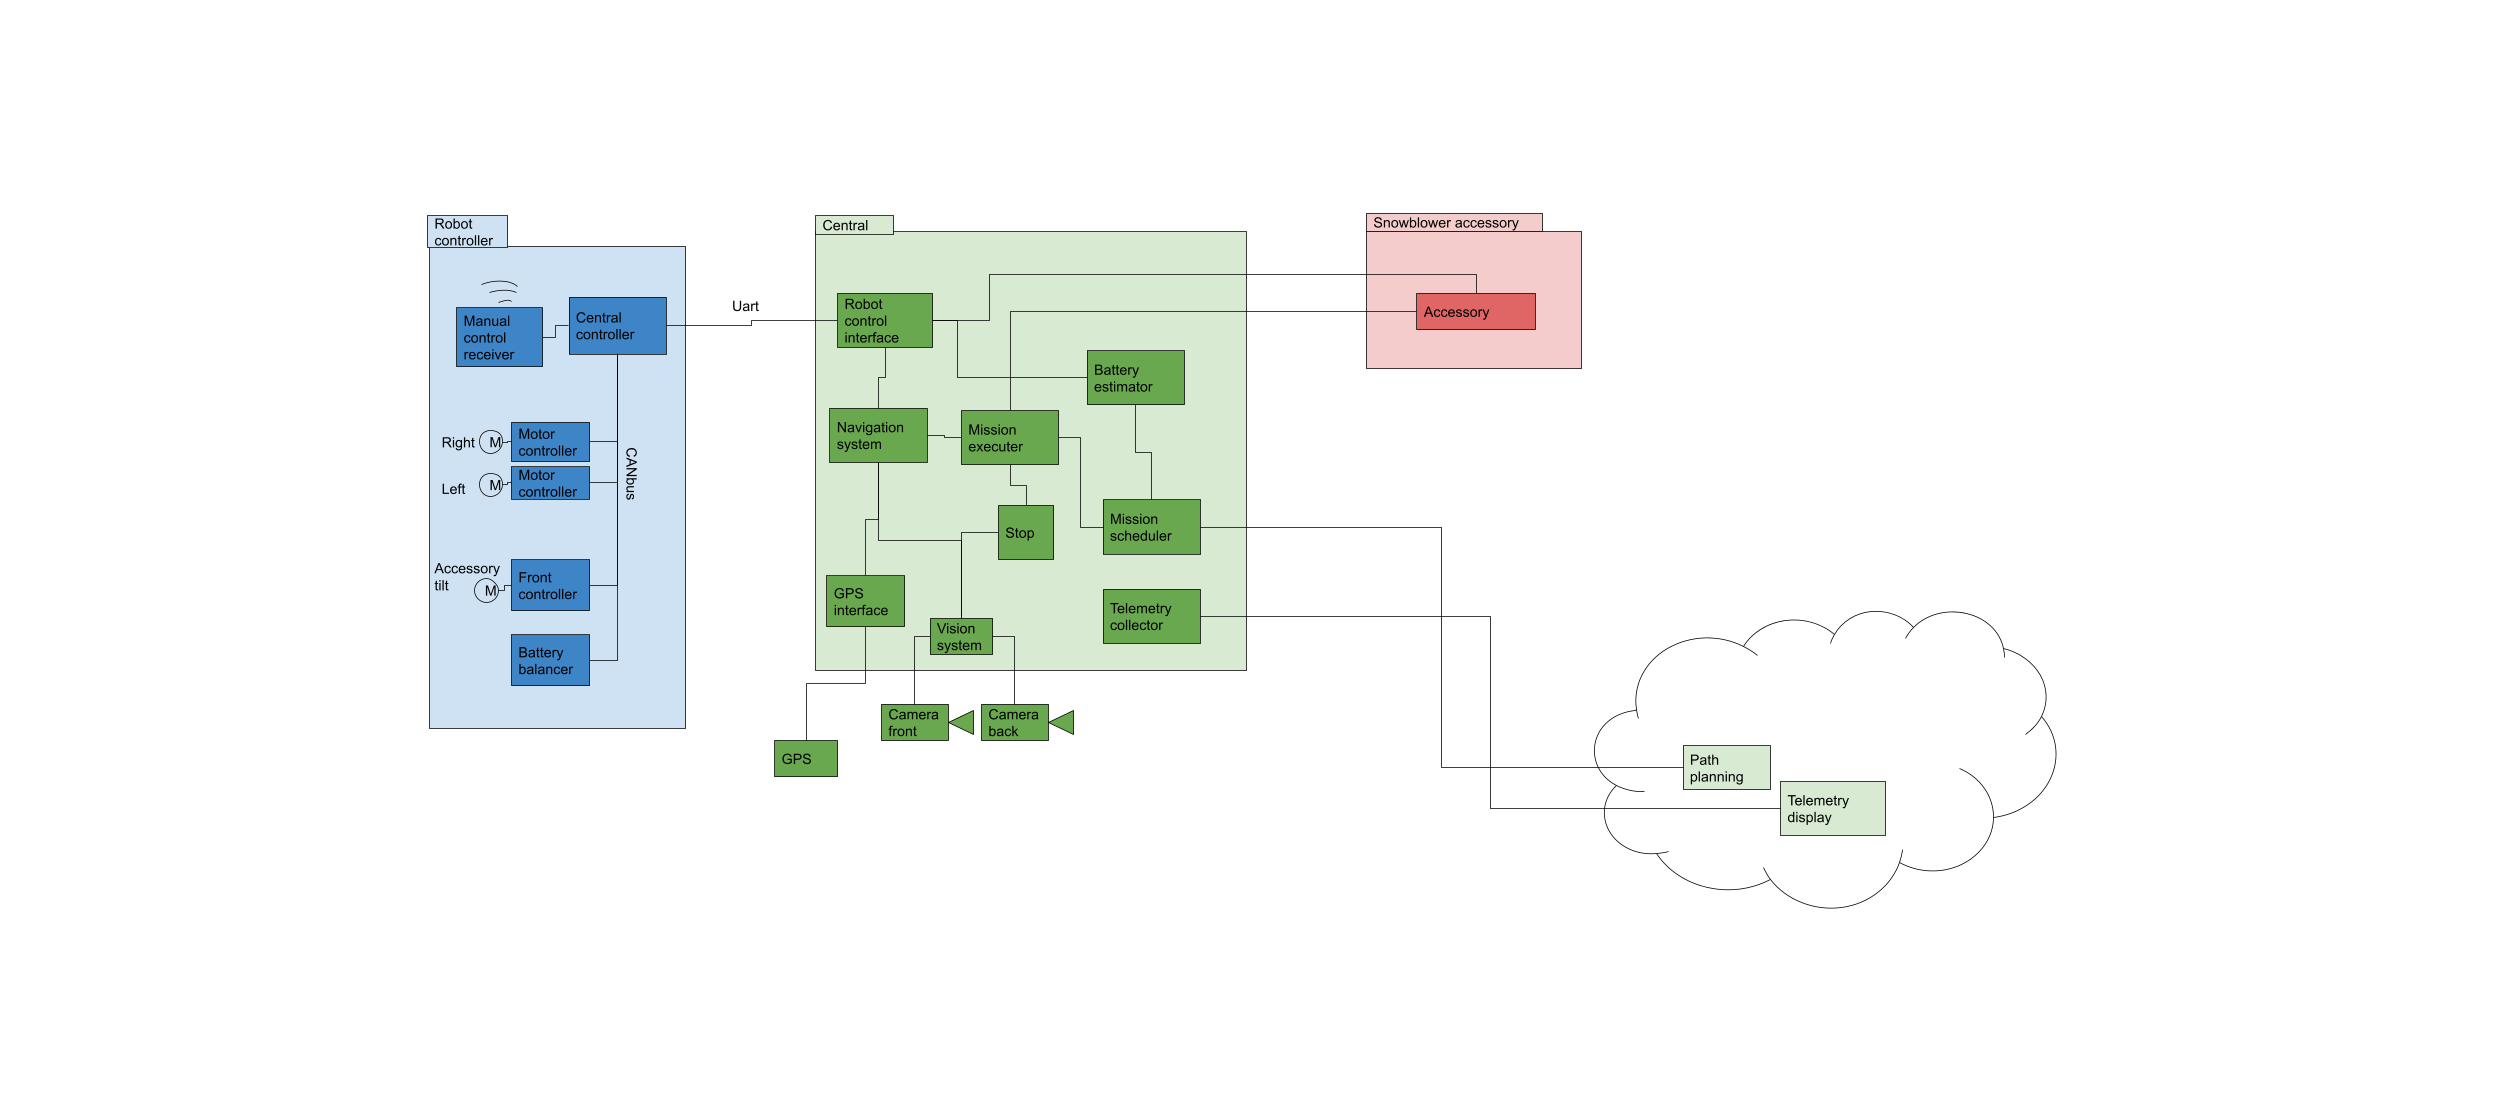
\includegraphics[width=\textwidth]{software_overview.png}
    \caption{Overview of the software architecture.}
    \label{fig:software_overview}
\end{figure}

The design of the software system is made up of different parts and are shown in figure \ref{fig:software_overview}. 
In figure \ref{fig:software_overview} each system is symbolized by a square with a describing name and
line symbolize communication between systems. Some communication lines are omitted for clarity,
what other system each system communicates with is described in the more detailed description of the system design.



\subsection{Design of all the parts}

\subsubsection{Mission scheduler}

\subsubsection{Mission executor}

\end{document}